\begin{figure*}[t]
  \centering
  \resizebox{\linewidth}{!}{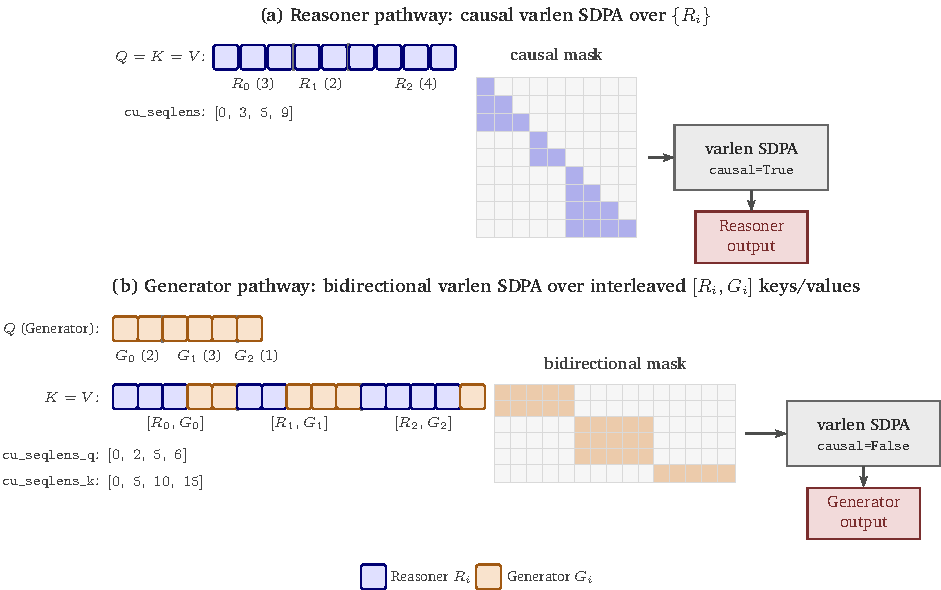
\includegraphics{figures/infrastructure/tikz_two_way_attention.pdf}}
  \captionsetup{justification=raggedright, singlelinecheck=false}
  \caption{\textbf{Two-way flat attention.} Each pathway is implemented as a single
  variable-length SDPA call. \textbf{(a)}~The Reasoner pathway uses a standard causal
  \texttt{varlen} call on the packed Reasoner tokens, producing a block-diagonal
  causal mask. \textbf{(b)}~The Generator pathway packs Generator queries separately
  from the interleaved key/value stream $[R_0, G_0, R_1, G_1, \ldots, R_n, G_n]$. The
  resulting mask is block-diagonal but rectangular within each block, so that each
  Generator query attends bidirectionally over its own sample's $[R_i, G_i]$ context
  without crossing sample boundaries. The example uses three packed samples with
  $(|R_i|, |G_i|) = (3, 2),\,(2, 3),\,(4, 1)$.}
  \label{fig:two_way_attention}
  \vspace{-0.5\baselineskip}
\end{figure*}
